\documentclass[times, utf8, seminar, numeric]{fer}
\usepackage[utf8]{inputenc}
\usepackage[T1]{fontenc}
\usepackage{currvita}
\usepackage{graphicx}
\usepackage{epstopdf}
\usepackage{listings}
\usepackage{textcomp}
\usepackage{booktabs}
\usepackage{algorithmic}
\usepackage{algorithm}


% definicija jezika koji nema nista, pa se nista ne naglasava
% koristi se za troadresni kod, ispise tokena i slicno
\lstdefinelanguage{blank}{
	sensitive=false, 
	morecomment=[l]{;},
}

% koristimo zadebljane vektore, a ne strelice
\renewcommand{\vec}[1]{\mathbf{#1}}

% prikazivanje shell naredbi
% http://tex.stackexchange.com/a/46962
\newcommand{\shellcmd}[1]{\\\indent\indent\texttt{\footnotesize\# #1}\\}

% neke boje koje koristimo u formatiranju ispisa
\usepackage{color}
\definecolor{mygreen}{rgb}{0,0.6,0}
\definecolor{mylightgray}{rgb}{0.95,0.95,0.95}

% definicija formatiranja ispisa, ponesto promjenjena u odnosu na pretpostavljenu
\lstset{ %
  backgroundcolor=\color{mylightgray},   % choose the background color; you must add \usepackage{color} or \usepackage{xcolor}
  basicstyle=\footnotesize\ttfamily,        % the size of the fonts that are used for the code
  breakatwhitespace=false,         % sets if automatic breaks should only happen at whitespace
  breaklines=true,                 % sets automatic line breaking
  captionpos=b,                    % sets the caption-position to bottom
  commentstyle=\color{mygreen},    % comment style
  deletekeywords={...},            % if you want to delete keywords from the given language
  escapeinside={\%*}{*)},          % if you want to add LaTeX within your code
  extendedchars=true,              % lets you use non-ASCII characters; for 8-bits encodings only, does not work with UTF-8
  frame=none,                    % adds a frame around the code
  keepspaces=true,                 % keeps spaces in text, useful for keeping indentation of code (possibly needs columns=flexible)
  keywordstyle=\color{blue},       % keyword style
  language=c,           	       % the language of the code
  morekeywords={*,...},            % if you want to add more keywords to the set
  numbers=none,                    % where to put the line-numbers; possible values are (none, left, right)
  numbersep=5pt,                   % how far the line-numbers are from the code
  numberstyle=\tiny\color{gray}, % the style that is used for the line-numbers
  rulecolor=\color{black},         % if not set, the frame-color may be changed on line-breaks within not-black text (e.g. comments (green here))
  showspaces=false,                % show spaces everywhere adding particular underscores; it overrides 'showstringspaces'
  showstringspaces=false,          % underline spaces within strings only
  showtabs=false,                  % show tabs within strings adding particular underscores
  stepnumber=2,                    % the step between two line-numbers. If it's 1, each line will be numbered
  stringstyle=\color{red},     % string literal style
  tabsize=2,                       % sets default tabsize to 2 spaces
  title=\lstname                   % show the filename of files included with \lstinputlisting; also try caption instead of title
}

\title{Implementacija FM-indeks algoritma}

\author{Ivan Borko, Sofia Čolaković, Florijan Stamenković}

\voditelj{doc. dr. sc. Mirjana Domazet Lošo}


\begin{document}

\maketitle

\tableofcontents

\chapter{Uvod i problematika}

Pretraživanje teksta česta je praktična potreba mnogih informacijskih sustava.
Pod terminom "pretraživanje teksta" podrazumijevamo pronalazak svih pojavljivanja
nekog niza znakova \textit{Q} \engl{query} unutar drugog niza znakova \textit{S} \engl{string}.
Tipično se rezultat pretraživanja \textit{R}
formulira kao niz indeksa (rednog broja znaka) unutar niza \textit{S} na kojem počinje pojavljivanje
niza \textit{Q}. Primjerice, za niz \textit{S = "Žuti pas je opasan kad je opasan remenom oko pasa"}
i niz \textit{Q = "pas"} rezultati
pretraživanja su \textit{R = \{6, 14, 28, 46\}}.

U području bioinformatike pretraživanje teksta koristi se za pronalazak
sekvenci unutar zadanog genoma. Definicija pretraživanja je jednaka. Specifičnost
bioinformatičkog pretraživanja jest da su nizovi koji se pretražuju iznimno velike duljine.
Primjerice, ljudski genom tipično sadrži oko $3.3 \times 10^9$ znakova, što bi otisnuto na
A4 stranice fontom veličine 10pt rezultiralo s otprilike milijun stranica.

Postoje mnogi algoritmi pretraživanja teksta
koji na jednostavan način ispunjavaju definirane zahtjeve.
Iz perspektive računalne složenosti algoritama, nije teško implementirati pretraživanje
teksta koje radi u linearnom vremenu\footnote{Ako nije drukčije navedeno pri razmatranju složenosti pretraživanja
uvijek govorimo o složenosti s obzirom na duljinu pretraživanog niza \textit{S}.}.
Nažalost, za nizove vrlo velike duljine linearno vrijeme
znači praktično predugo trajanje pretraživanja. Otud potreba, pogotovo u području bioinformatike,
za vremenski sub-linearnim algoritmima pretraživanja. Istovremeno, potrebno je memorijske
zahtjeve algoritma pretraživanja zadržati što manjima.

U ovom projektu razmatramo implementaciju pretraživanja teksta koja se bazira na konceptu
FM-indeksa. Konkretna implementacija bazira se na binarnim stablima valića \engl{wavelet-trees}.
Teoretsko razmatranje i praktično testiranje pokazuju da ovakva implementacija pretraživanja
ima vremenski sub-linearnu složenost, uz prihvatljivu memorijsku složenost.

\chapter{FM-indeks algoritam}

"Indeksiranje" teksta označava generiranje struktura podataka koje su podrška efikasnom
pretraživanju. Za velike tekstove poželjno je da indeks bude memorijski efikasan.
FM-indeks \cite{Ferragina00opportunisticdata} pristup je indeksiranju koji ispunjava
zahtjeve memorijske efikasnosti i sub-linearnog vremena pretraživanja. Prije nego definiramo
FM-indeks, potrebno je razmotriti podatkovne strukture i algoritme koji ga sačinjavaju.

\section{Burrows-Wheeler transformacija (BWT)}

Burrows-Wheeler transformacija \cite{btw_1994} transformira niz znakova na način koji
će omogućiti efikasnu pohranu i brzo ptreživanje. BWT transformirani niz originalnog
teksta \textit{T} označavati ćemo sa \textit{T\textsuperscript{BTW}}. Transformacija se provodi sljedećim koracima:

\begin{enumerate}
  \item{Poseban znak '\$' koji je leksikografski manji od svih ostalih znakova se dodaje na kraj niza \textit{T}}
  \item{Cikličkim rotacijama niza \textit{T} dobiva sa se skup nizova koji čini tablicu \textit{CR} \engl{cyclic rotation}}
  \item{Tablica \textit{CR} se leksikografski sortira u tablicu \textit{SCR}}
  \item{Posljednji stupac tablice \textit{SCR} (čitan odozgo prema dolje) čini rezultat \textit{T\textsuperscript{BTW}}}
\end{enumerate}

Opisani postupak ilustriran je za niz \textit{T = "AGATTAT"} na slici \ref{fig:bwt}, preuzetoj iz rada
\cite{singer_2012}.

\begin{figure}[!htb]
\centering
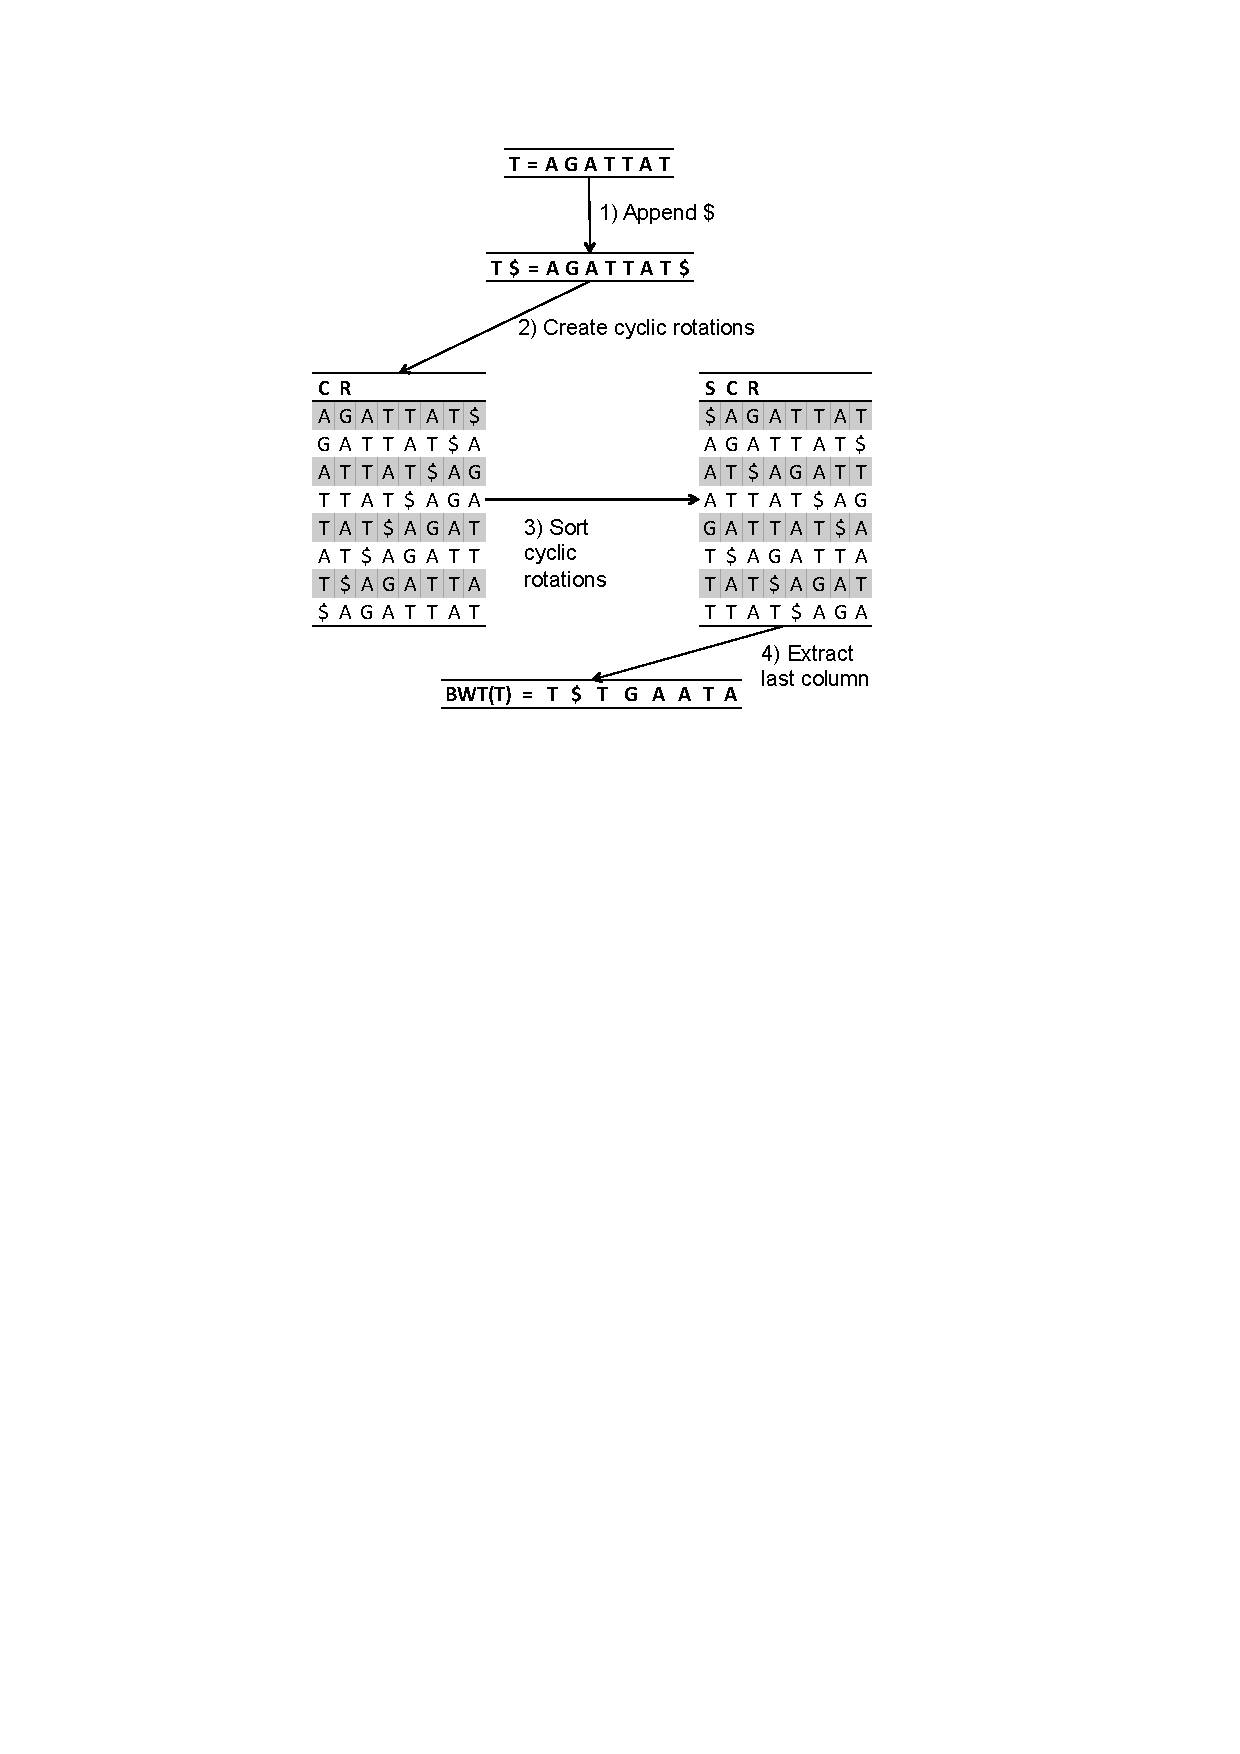
\includegraphics{fig/bwt.pdf}
\caption{Primjer algoritma BWT transormacije niza \textit{T = AGATTAT}}
\label{fig:bwt}
\end{figure}

Bitno je primjetiti kako je BWT transformacija niza srodna sufiksnoj listi \textit{SA} \engl{suffix array}. Sufiksna lista
je struktura podataka koja se često koristi u algoritmima nad tekstom. Njenu formulaciju
nećemo detaljno objašnjavati, materijali na temu su široko dostupni. Sličnost između BWT
transformacije i \textit{SCR} tablice korištene u BWT transformaciji ilustrirana je slikom \ref{fig:bwt_sa}.

\begin{figure}[!htb]
\centering
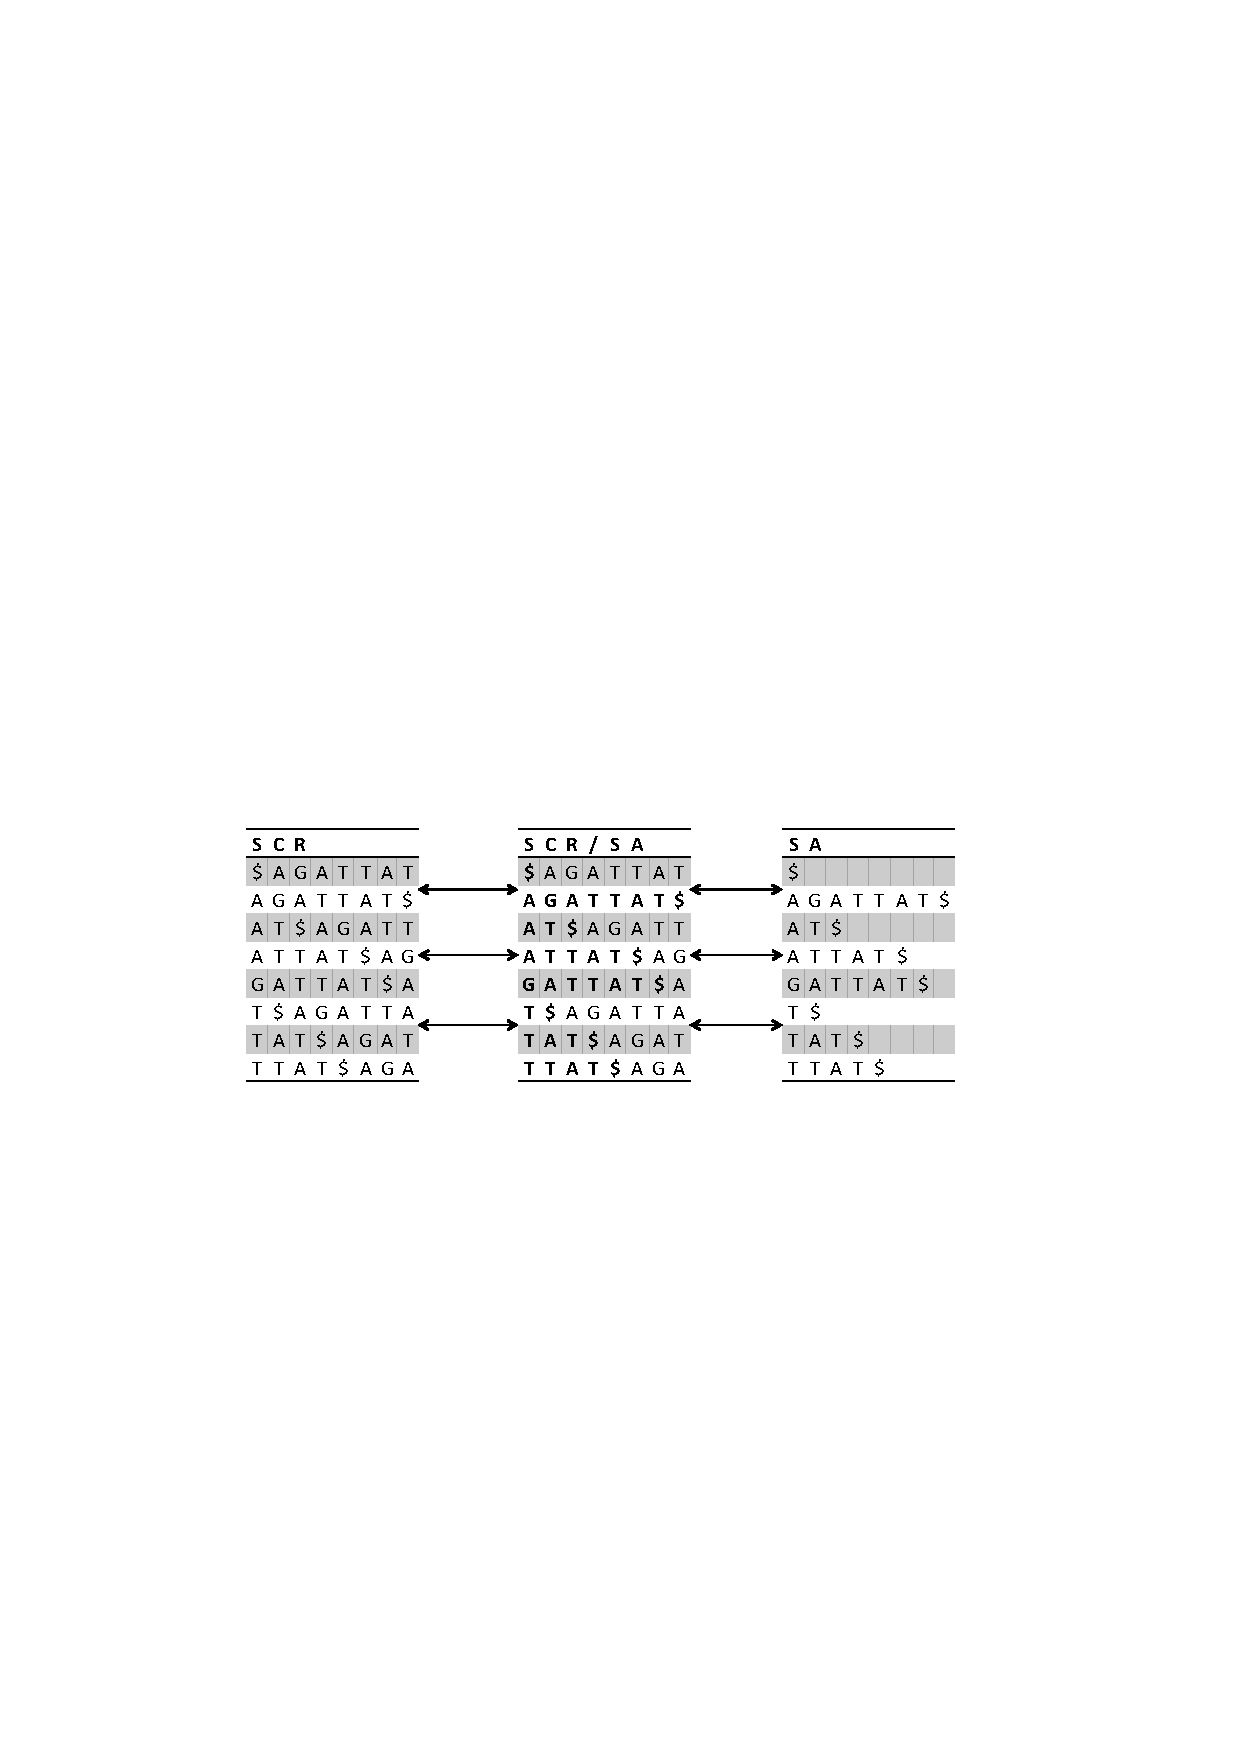
\includegraphics{fig/bwt_sa.pdf}
\caption{SCR tablica BWT tranfsformacije i sufiksna lista za niz \textit{T = AGATTAT}}
\label{fig:bwt_sa}
\end{figure}

\subsection{LF-mapiranje}

LF-mapiranje \engl{last-to-first mapping} opisuje relaciju između posljednjeg
stupca \textit{SCR} tablice (označenog \textit{L}) i prvog stupca te iste tablice (označenog
\textit{F})\footnote{Primjetimo da je \textit{L} isti stupac
koji definira BWT transformaciju.}. LF-mapiranje postulira da
\textit{i}-to pojavljivanje znaka \textit{c} unutar stupca \textit{L} korespondira
\textit{i}-tom pojavljivanju tog istog znaka unutar stupca \textit{F}. Pri tome "korespondira"
znači da se radi o istom znaku unutar originalnog niza \textit{T}. Jednostavan dokaz ovog
iskaza moguće je naći u \cite{singer_2012}.

Brza implementacija LF-mapiranja (konstantne
vremenske složenosti) može se ostvariti korištenjem dviju pomoćnih tablica. Tablica
prefiksnih suma \textit{C} \engl{prefix-sum table} niza \textit{T} za svaki znak \textit{c}
pohranjuje broj znakova u \textit{T} koji su manji od \textit{c}. Tablica pojavljivanja
\textit{Occ} \engl{occurrence table} pohranjuje informaciju koliko puta se neki znak
\textit{c} pojavio u nizu \textit{T} do pozicije \textit{i} (isključujući znak točno na
poziciji \textit{i}). Korištenjem tablica \textit{C} i \textit{Occ} LF-mapiranje za
\textit{T\textsuperscript{BWT}} (koji odgovara stupcu \textit{L}) računa se na sljedeći način,
za znak \textit{c} na poziciji \textit{i}:

\begin{enumerate}
  \item{Pronađi broj pojavljivanja \textit{c} u \textit{T\textsuperscript{BWT}} do pozicije \textit{i} unutar tablice \textit{Occ}}
  \item{Pronađi broj znakova manjih od \textit{c} u \textit{T\textsuperscript{BWT}} unutar tablice \textit{C}}
  \item{Zbroj pronađenih vrijednosti je indeks korespondirajućeg znaka u stupcu \textit{L}}
\end{enumerate}

\subsection{Rekonstrukcija originala}

Na temelju transformiranog niza \textit{T\textsuperscript{BWT}} moguće je rekonstruirati
originalni niz \textit{T} korištenjem LF-transformacije. Postupak je jednostavan, ako imamo
na umu definiciju LF-transformacije i činjenicu da je prvi znak u \textit{T\textsuperscript{BWT}}
zasigurno posljednji znak niza \textit{T} (ovo proizlazi iz činjenice da smo pri postupku BWT
transormacije na početak niza umetnuli znak '\$').

Rekonstrukcija niza \textit{T} obavlja se unatrag, od posljednjeg znaka prema prvom. Postupak
je sljedeći:

\begin{enumerate}
  \item{Prvi znak iz \textit{T\textsuperscript{BWT}} je posljednji znak iz \textit{T}, zabilježimo ga}
  \item{LF-transformacijom pronađimo \textit{F}-indeks  posljednjeg zabilježenog znaka \footnote{
    U ovom trenutku nemamo tablicu \textit{SCR} niti stupac \textit{F}, zanima nas samo indeks.}}
  \item{Dobiveni \textit{F}-indeks u \textit{T\textsuperscript{BWT}} nizu ukazuje na znak koji u nizu
    \textit{T} prethodi posljednjem zabilježenom znaku (posljedica rotacije pri konstrukciji \textit{SCR})}
  \item{Zabilježimo znak na \textit{F}-indeks poziciji niza \textit{T\textsuperscript{BWT}} u rekonstrukciju}
  \item{Ako posljednji zabilježeni znak nije '\$', vraćamo se na korak 2.}
\end{enumerate}

Opisani postupak vizualiziran je na slici \ref{fig:lf_reconstruct}. Bitno je primjetiti kako pri
rekonstrukciji originala nismo koristili ništa osim transformiranog niza \textit{T\textsuperscript{BWT}}
i LF-mapiranja (koje se ostvaruje tablicama \textit{C} i \textit{Occ}).

\begin{figure}[!htb]
\centering
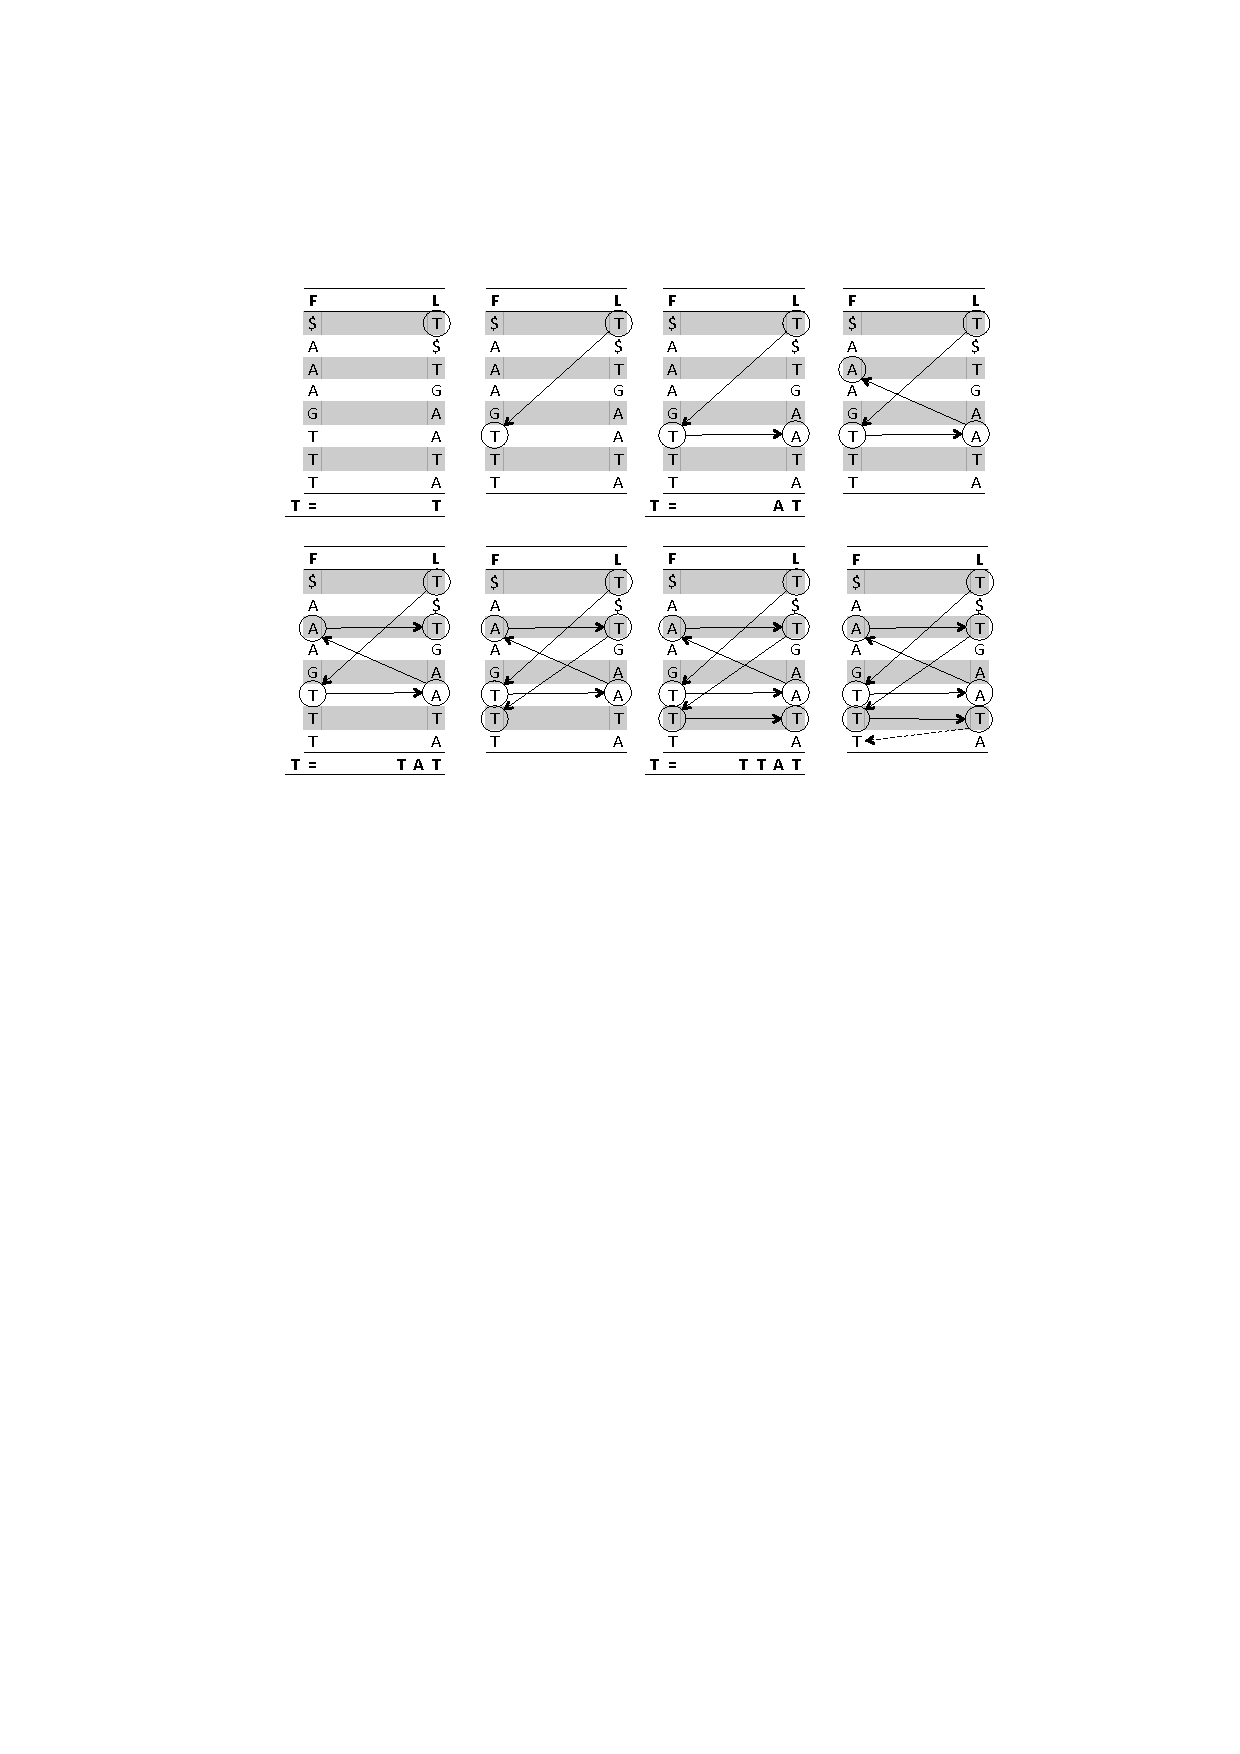
\includegraphics{fig/lf_reconstruct.pdf}
\caption{Primjer rekonstrukcije originala iz transformiranog niza \textit{T\textsuperscript{BWT}}}
\label{fig:lf_reconstruct}
\end{figure}

\subsection{Pretraživanje}
\label{sec:pretrazivanje}

Transformirani niz \textit{T\textsuperscript{BWT}} može se koristiti i za pretraživanje
originalnog teksta \textit{T}. Algoritam pretraživanja vrlo je sličan rekonstrukciji
originala. Bazira se zapravo na poznatom načinu pretraživanja sufiksnih polja. Kao
što je već spomenuto, BWT transformacija i sufiksno polje nekog niza su skoro ekvivalentni.

Algoritam pretraživanja pojavljivanja niza \textit{Q} unutar niza \textit{T} na temelju
BWT transforacije \textit{T\textsuperscript{BWT}} bazira se na sljedećim konceptima:

\begin{itemize}
  \item{Pretraživanje se vrši po znakovima \textit{Q} unatrag (od zadnjeg prema prvom)}
  \item{Prate se početni i krajnji indeks sufiksa (\textit{SCR} tablice) unutar kojih su moguće podudarnosti}
  \item{U svakom koraku (procesiranom znaku iz \textit{P}) se područje mogućih podudarnosti smanjuje}
\end{itemize}

Ako početni indeks označimo \textit{ps} \engl{pointer start}, a krajnji indeks \textit{pe}
\engl{pointer end}, tada se algoritam izvršava sljedećim koracima:

\begin{enumerate}
  \item{Inicijaliziraj indekse \textit{ps} i \textit{pe} tako da obuhvaćaju cijelu tablicu \textit{SCR}}
  \item{Odaberi prvi neobrađeni znak \textit{c} iz niza \textit{Q}, počevši od kraja}
  \item{Unutar područja među indeksima nađi prvo i posljednje pojavljivanje znaka \textit{c}
    \footnote{Učinkovita implementacija pretraživanja ne izvršava ovaj korak, navodimo ga
    samo radi opisa rada algoritma.}}
  \item{Izračunaj \textit{L}-indekse nađenih pojavljivanja koristeći LF-mapiranje}
  \item{Dobiveni \textit{L}-indeksi su nove vrijednost indeksa \textit{ps} i \textit{pe}}
  \item{Ako postoje neobrađeni znakovi u \textit{Q}, vrati se na korak 2.}
\end{enumerate}

Navedeni koraci algoritma formulirani su kako bi bili što jasniji. Opis prikladniji
za izravnu računalnu implementaciju može se naći u radu \cite{singer_2012}. Slika
\ref{fig:sa_search} prikazuje korake pretraživanja za \textit{Q = TAT}.

\begin{figure}[!htb]
\centering
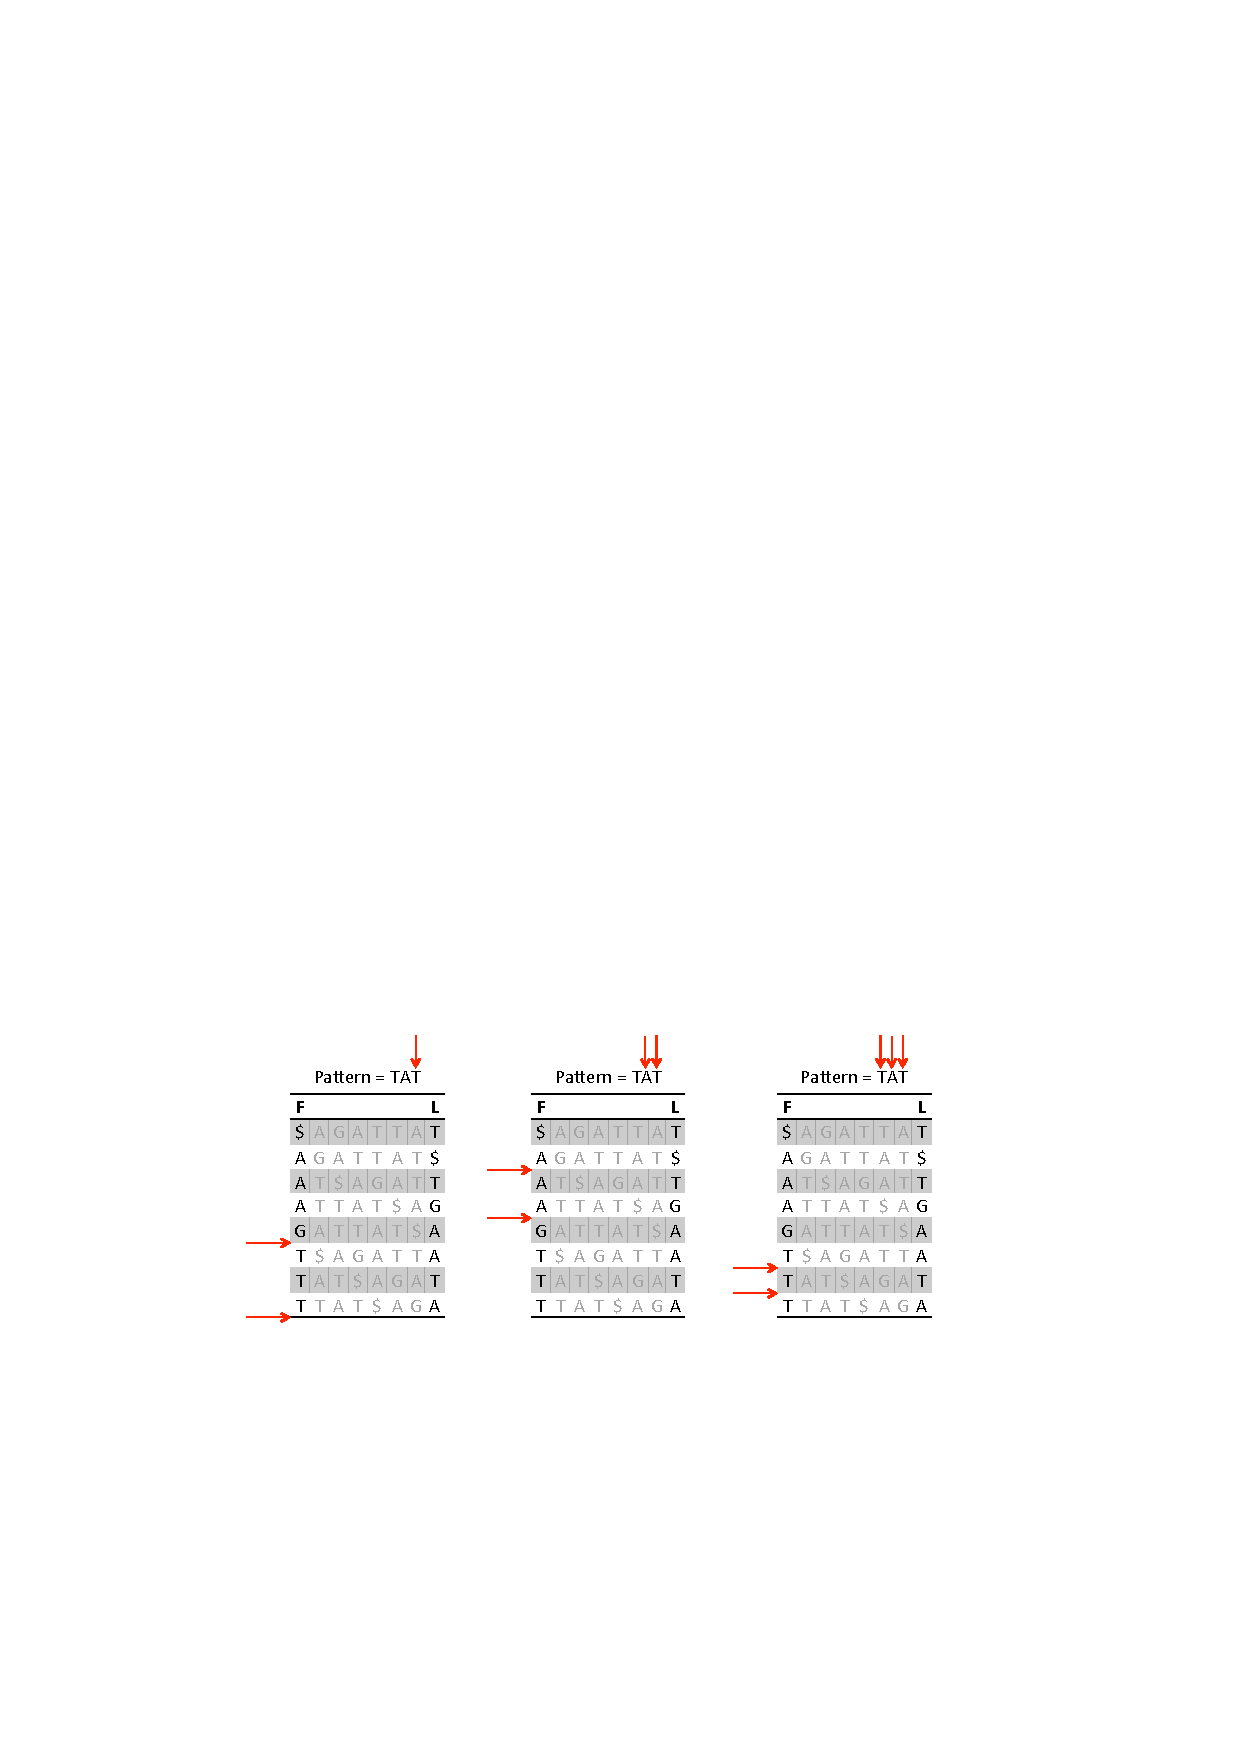
\includegraphics{fig/sa_search.pdf}
\caption{Primjer pretraživanja teksta korištenjem transformiranog niza \textit{T\textsuperscript{BWT}}}
\label{fig:sa_search}
\end{figure}

\section{Složenost pretraživanja}

Glavni razlog za razvoj FM-indeksa je povećanje efikasnosti pretraživanja dugih nizova
(poput genotipa). U ovom poglavlju će se razmotriti teoretska složenost pretraživanja korištenjem
FM-indeksa. Pri tome nas zanima složenost korištenja
izgrađenog indeksa za neki niz, a ne složenost stvaranja indeksa.

\subsection{Vremenska složenost}

Razmotrimo vrijeme pronalaska pojavljivanja niza \textit{Q} unutar niza \textit{T}, na
način opisan u poglavlju \ref{sec:pretrazivanje}. Iz algoritma je vidljivo da je
potreban jedan korak za svaki znak u \textit{Q}, dakle pretraživanje ima linearnu
složenost s obzirom na duljinu \textit{Q}. Svaki od tih koraka svodi se na dvije
operacije LF-mapiranja, koje ima konstantnu vremensku složenost (ne ovisi o duljinama
nizova \textit{T} i \textit{Q}).

Važna napomena je da prolazak kroz znakove niza \textit{Q} može biti prekinut u slučaju
da se utvrdi da nema pojavljivanja \textit{Q} unutar \textit{T}, što se može desiti
u bilo kojem trenutku prolaska kroz \textit{Q}.

Dakle, vremenska složenost pretraživanja je generalno linearna s obzirom na duljinu
niza \textit{Q}. Ovaj rezultat je pogodan za pretraživanje dugih nizova \textit{T},
jer ne ovisi o njihovoj duljini.

\subsection{Memorijska složenost}

Memorijska (prostorna) složenost označava utrošak memorije na potporne
strukture podataka FM-indeksa, s obzirom na niz \textit{T}.
Podatkovne strukture koje se koriste u pretraživanju su transformirani niz
\textit{T\textsuperscript{BWT}} (odnosno sufiksno polje) te tablice \textit{C}
i \textit{Occ} korištene za LF-mapiranje.

Sufiksno polje ima jednak broj elemenata kao i originalni niz \textit{T}. U
tom smislu je memorijska složenost polja linearna s obzirom na duljinu \textit{T}.
Isto vrijedi i za transformirani niz \textit{T\textsuperscript{BWT}}. Prostorni
utrošak sufiksnog polja može se smanjiti na više načina, a niz \textit{T\textsuperscript{BWT}}
je često oblika pogodnog za komprimiranje. Obje tehnike izlaze izvan okvira
ovog rada, mi koristimo postojeće implementacije sufiksnog polja koje su memorijski
optimizirane.

Tablica prefiksnih suma \textit{C} pohranjuje po jedan cijeli broj za svaki
element abecede niza \textit{T}. Iako je u teoriji broj znakova abecede ograničen samo
duljinom niza \textit{T}, u praksi je najčešće vrlo malen te tablica \textit{C}
ne predstavlja problem u kontekstu zauzeća memorije.

Tablica pojavljivanja \textit{Occ} (u naivnoj implementaciji) pohranjuje po
jedan cijeli broj za svaku poziciju niza \textit{T}, za svaki element abecede \textit{T}.
Primjećujemo linearnu složenost s obzirom na duljinu niza \textit{T}. S obzirom
na potencijalno ogromne duljine nizova koje želimo moći pretraživati, ovo je problem.
Postoji više pristupa "kodiranja" tablice \textit{Occ}. Unutar ovog rada, zadatak
je implementirati FM-indeks korištenjem stabla valića.


\chapter{Stablo valića}

Stablo valića \engl{wavelet tree}, definirano u \cite{Grossi:2003:HET:644108.644250},
koristimo za efikasnu implementaciju 
tablice pojavljivanja \textit{Occ}, koja se koristi za LF-mapiranje unutar
FM-indeksa. \textit{Occ} tablica daje informaciju o broju
pojavljivanja znaka \textit{c} unutar niza \textit{T} do pozicije \textit{i}
(ne uključujući znak na poziciji \textit{i}). Ova operacija naziva se "rangiranje",
možemo reći da tražimo \textit{rank} znaka \textit{c} u \textit{T} do pozicije \textit{i},
odnosno \textit{rank(T, c, i)}.

\section{Definicija stabla valića}

Stablo valića kodira niz \textit{T} u binarno stablo. Svaki čvor stabla ima pripadajući
znak (prijelomnu točku \textit{p}) i binarni niz (niz sačinjen od nula i jedinica). Nule u 
binarnom nizu čvora označavaju znakove
originalnog niza koji su manji od znaka prijelomne točke \textit{p}, a jedinice
znakove koji su veći ili jednaki (pri tome se u čvoru ne pohranjuje originalni niz, već
samo binarni). Znakovi originalnog niza označeni nulama sačinjavaju lijevo
dijete čvora, a oni označeni jedinicama desno. Čvorovi se kreiraju samo ako sadrže dva ili više
različita znaka (za niz proizvoljne duljine začinjen od samo jednog znaka se ne stvara stablo).
 Primjer binarnog stabla za genotipski niz "AGCTAGCTCATACAGGGTATGACCAGTACGACAG"
prikazan je na slici \ref{fig:wavelet_ex1}.

\begin{figure}[!htb]
\centering
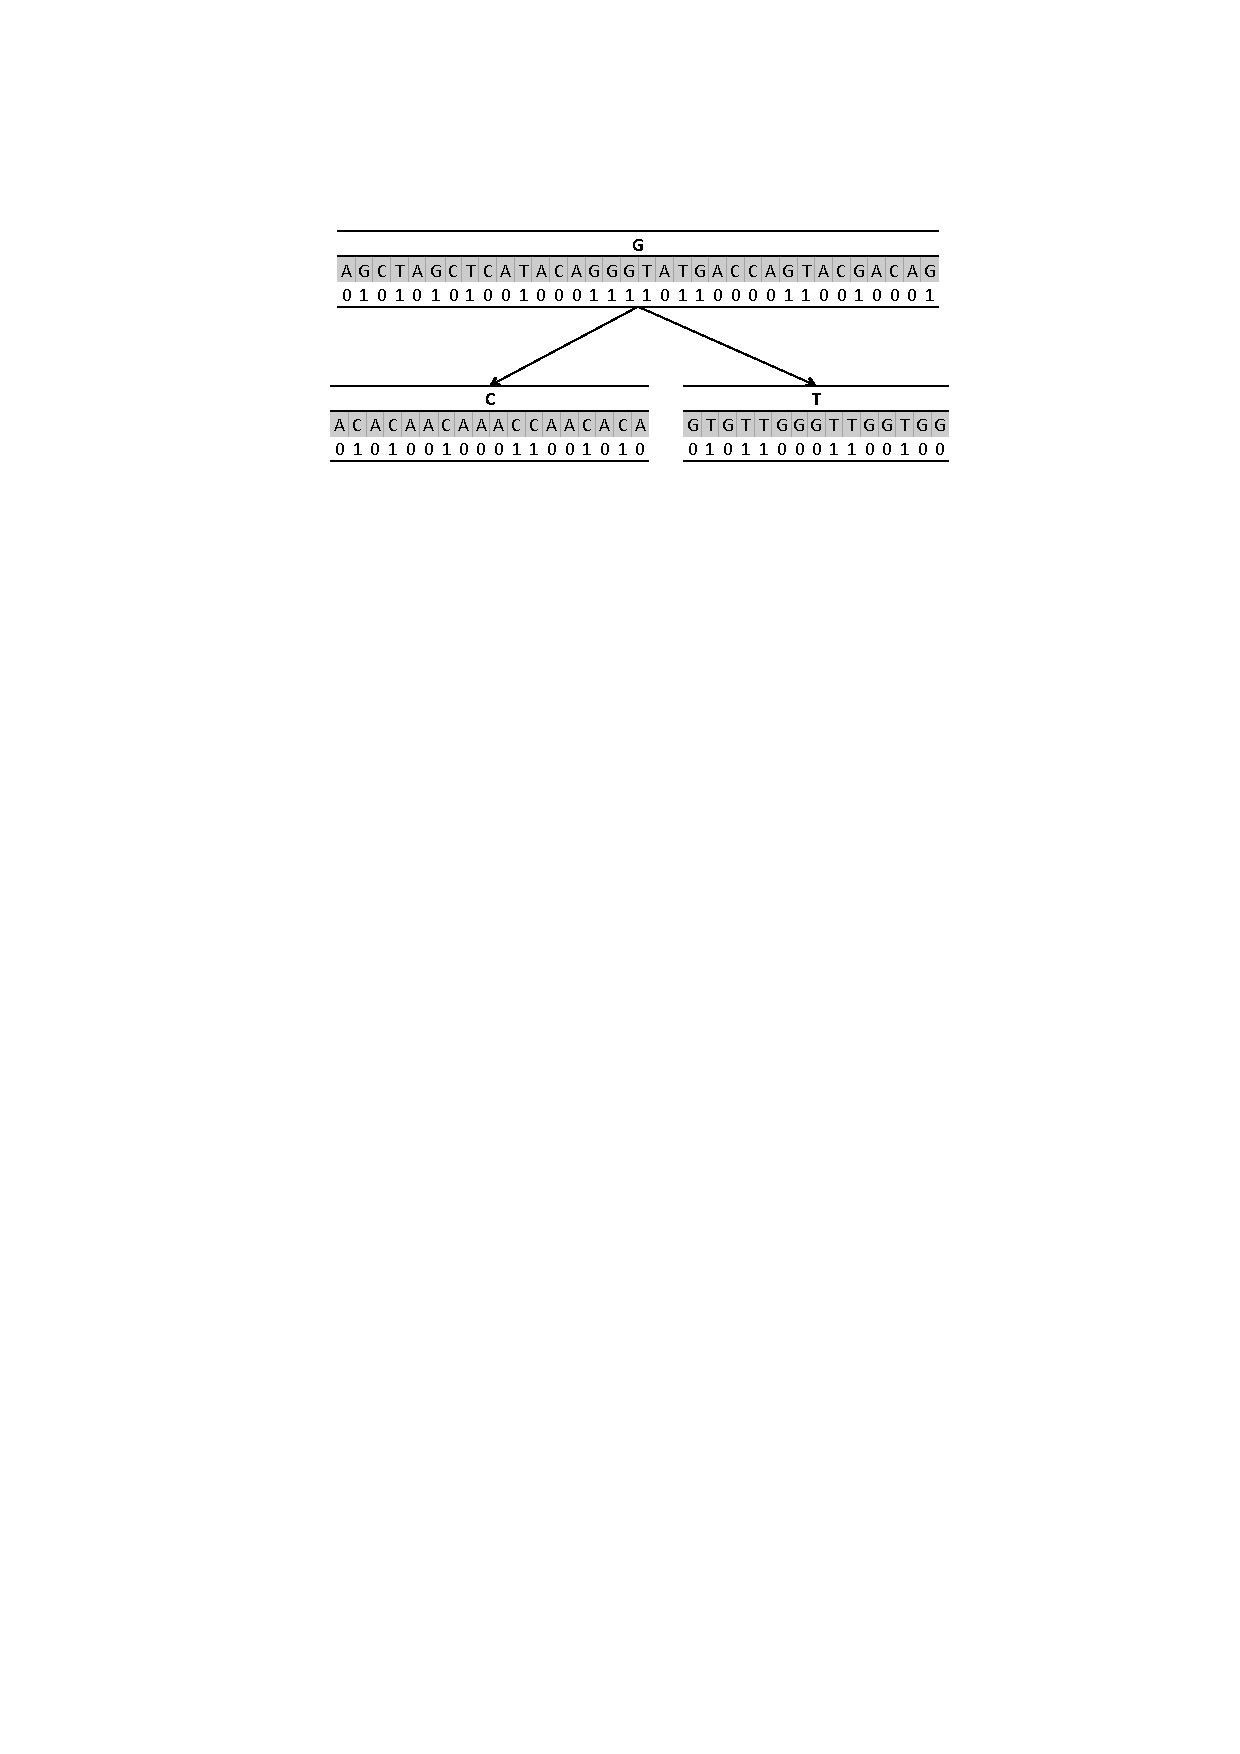
\includegraphics{fig/wavelet_ex1.pdf}
\caption{Primjer stabla valića za niz "AGCTAGCTCATACAGGGTATGACCAGTACGACAG". Znakovi
  originalnog niza prikazani u čvorovima stabla služe samo za ilustraciju, konkretna implementacija
  sadrži samo binarne nizove i znakove koji su prijelomne točke čvorova.}
\label{fig:wavelet_ex1}
\end{figure}

\section{Rangiranje korištenjem stabla valića}

"Rank" znaka \textit{c} unutar niza \textit{T} do pozicije \textit{i} je broj pojavljivanja
tog istog znaka u prvih \textit{i} znakova niza \textit{T}. Operacija rangiranja može
se efikasno ostvariti korištenjem stabla valića.

Pretpostavimo da imamo
vremenski konstantnu implementaciju binarnog rangiranja. Binarno rangiranje ima
istu definiciju kao općenito rangiranje, ali se obavlja nad binarnim nizovima,
dakle svodi se na prebrojavanje jedinica u binarnom nizu. Implementacija
vremenski konstantne složenosti biti će objašnjena u nastavku. 

Svaki čvor stabla ima pripadnu prijelomnu točku \textit{p} i binarni niz.
Koristeći binarno rangiranje
za svaki čvor stabla valića lako je utvrditi broj znakova manjih ili većih
od \textit{p}, u prvih \textit{i} znakova čvora. Razmatramo dvije situacije:
znak \textit{c} koji rangiramo može biti leksikografski manji od \textit{p}
ili veći-ili-jednak. U prvoj situaciji broj nula binarnog ranga čvora po
\textit{p} govori koliko znakova lijevog djeteta čvora trebamo pretražiti,
u drugoj situaciji broj jedinica govori koliko znakova desnog djeteta trebamo
pretražiti. Spuštajući se tako kroz stablo dolazi trenutak kada relevantno
dijete trenutnog čvora ne postoji, tada je trenutni broj pretraživanja istovremeno
i konačni rezultat. Opširnija objašnjenja rangiranja korištenjem stabla valića
široko su dostupna\footnote{Primjerice na http://alexbowe.com/wavelet-trees/}.

\section{Vremenska i memorijska složenost stabla valića}

\subsection{Vremenski konstantno binarno rangiranje}

Za ostvarivanje brzog rangiranja korištenjem stabla valića potrebna je sposobnost
brzog rangiranja binarnog niza. Problem rangiranja binarnog niza jednostavniji
je jer postoje samo dva znaka abecede. Pri tome je potrebno rangirati samo jedan
znak (primjerice znak 1) jer se rang drugog znaka dobiva kao \textit{rank(T, 0, i)
= i - rank(T, 1, i)}. Konstantna vremenska složenost ovakvog rangiranja ostvaruje
se grupiranjem niza u "kante" duljine \textit{k}. Za svaku kantu se prati broj
jedinica sadržanih u svim prethodnim kantama. Time se za svaki \textit{i} rangiranje
obavlja određivanjem kante kojoj \textit{i} pripada, običnim prebrojavanjem jedinica
do pozicije \textit{i} samo unutar
te kante, te pribrajanjem broja jedinica sadržanih u prethodnim kantama. Time je
prebrojavanje (iteracija po znakovima) ograničeno na veličinu kante, ne ovisi više
o duljini originalnog niza. Ovakvo rangiranje stoga ima konstantnu vremensku složenost s obzirom
na duljinu originalnog niza.

Konkretna implementacija opisanog rangiranja je malo složenija jer se zbog
memorijske učinkovitosti koriste kante i "super-kante", ali je konceptualno
identična i vremenski jednako efikasna.

\subsection{Vremenska složenost rangiranja stablem valića}

Stablo valića može prestavljati proizvoljan niz, proizvoljne abecede. Pri tome
se ono razlaže binarno po elementima abecede. Rangiranje se svodi na jedan
dubinski prolaz kroz stablo. Dubina binarnog stabla je jednaka
$log_2(|\Sigma|)$, gdje je $\Sigma$ skup znakova abacede,
što istovremeno određuje vremensku složenost rangiranja. Pošto je
binarno rangiranje u svakom čvoru konstantne složenosti, konačna složenost
rangiranja je logaritamska s obzirom na veličinu abecede. Pošto su
u većini primjena korištene abecede relativno male (u bioinformatici radi
se o 4 ili 5 znakova), rangiranje korištenjem stabla valića ima iznimno
dobre performanse.

\subsection{Memorijska složenost stabla valića}

Indeksiranje niza znakova u pravilu povećava memorijsku složenost kako
bi se smanjila vremenska. Pri tome je poželjno da memorijsko povećanje
nije preveliko, pogotovo kada se radi sa iznimno velikim nizovima.

Stablo valića pohranjuje binarne varijante originalnog niza. Pri tome
korijenski čvor pohranjuje binarni niz dulje jednake originalnom nizu.
Djeca korijenskog čvora sadrže binarne nizove koji zajedno imaju duljinu
jednaku originalnom nizu (može se isčitati iz definicije, ilustrirano
na slici \ref{fig:wavelet_ex1}). Ista stvar se dešava sa daljnjim grananjem
stabla. Stoga svaka razina stabla (čvorevi jednako udaljeni od korijenskog)
sadrži binarne nizove čija ukupna duljina je jednaka originalnom nizu.
Stablo ima  $log_2(|\Sigma|)$ razina, gdje je $\Sigma$ skup znakova abacede.
Stoga je konačna memorijska složenost stabla $n * log_2(|\Sigma|)$ bitova, gdje
je $n$ broj znakova originalnog niza.
Sličnu složenost imaju neki algortmi kompresije, radi se dakle o
relativno niskoj memorijskoj zahtjevnosti.

\chapter{Implementacija i testiranje}

\section{Implementacija}

Zbog brzine izvođenja FM-indeks je implementiran u C++ programskom jeziku, osim skripti za pokretanje generiranja sintetskih podataka i samih skripti za generiranje sintetskih podataka, koje su pisane u \textit{bash}-u, odnosno \textit{pythonu} verzije 2.
Pojedini algoritmi su prije toga izvedeni i u Python programskom jeziku, radi
jednostavnosti implementacije i testiranja, te potom optimalno prevedeni u
C++. C++ kod smo prevodili pomoću \texttt{gcc} prevodioca verzije 4.9, koji je praktički standard na \textit{unix} okruženjima. Kod prevođenja je korištena naredba \textit{-O2} prevodica.

Implementacija se sastoji od BW-transformacije i potpornih struktura za LF-mapiranje.
Pri tome je tablica prefiksnih suma \textit{C} implementirana trivijalno (ništa
drugo nije potrebno), a tablica pojavljivanja \textit{Occ} je implementirana
trivijalno i u obliku stabla valića. Korištena je postojeća implementacija sufiksnog
polja\footnote{https://sites.google.com/site/yuta256/sais}. Napisani su UnitTestovi
pojedinih funkcionalnosti, kao i testovi za cjelokupni FM-indeks, što uključuje
evaluaciju vremenske i memorijske složenosti pretraživanja.

Cijeli kod je objavljen na javnom \textit{GitHub} repozitoriju, na adresi \url{https://github.com/iborko/fmindex}. Cijeli kod se može preuzeti naredbom:
\shellcmd{git clone --recursive https://github.com/iborko/fmindex}

Napisana je i \textit{makefile} datoteka koja ubrzava cijeli proces prevođenja te omogućava zasebnu izgradnju izvršne datoteke s testovima (\textit{test}) i izvršne datoteke sa samom implementacijom FM indeksa (\textit{fmindex}). Automatizirani proces prevođenja koristeći \textit{Makefile} alat se pokreće upisivanjem naredbe:
\shellcmd{make}
u korijenskom direktoriju repozitorija. Može se pozvati i zasebno prevođenje same implementacije:
\shellcmd{make fmindex}
ili samo testova:
\shellcmd{make test}

\noindent Nakon prevođenja izvršne će se datoteke nalaziti u mapi \texttt{bin}. Opis korištenja:
\shellcmd{fmindex <sequence> <reads> [<occurrence\_table> [<bucket\_size>]]}
\begin{description}
  \item[sequence] putanja do sekvence \engl{sequence} na kojoj se izvodi pretraživanje, u FASTA\footnote{http://en.wikipedia.org/wiki/FASTA\_format} formatu
  \item[reads] putanja do očitanja \engl{reads} koji će se tražiti u sekvenci, FASTQ\footnote{http://en.wikipedia.org/wiki/FASTQ\_format} formatu
  \item[occurrence\_table] može biti \textit{0} (trivijalna implementacija tablice pojavljivanja), \textit{1} (implementacija tablice pojavljivanja pomoću stabla valića)
  \item[bucket\_size] veličina kante kod implementacije stabla valića
\end{description}

\noindent Primjer pokretanja:
\shellcmd{fmindex Esch\_coli\_536.fna Esch\_coli\_536\_reads.fq 1 40}

Za svako očitanje iz \texttt{<reads>} datoteke, program generira dvije linije. Prva linija je header tog očitka iz \texttt{<reads>} datoteke, a druga linija je niz indeksa položaja tog očitka u \texttt{<sequence>} datoteci. Indeksi su odvojeni razmakom. Izlaz se ispisuje na standardni izlaz \engl{stdout}.

\section{Testiranje}

\subsection{Oblici testiranja}

UnitTestovi pojedinih funkcionalnosti (primjerice stabla valića i binarnog ranka) pisani su
kako bi se utvrdila njihova ispravnost. Pri tome se testiralo nad sintetiziranim,
nasumičnim podatcima. Uspoređuju se trivijalne implementacije (jednostavne za napisati,
ali vremenski i memorijski neefikasne) sa produkcijskim algoritmima. U trenutku pisanja
UnitTestovi indiciraju da su sve produkcijske funkcionalnosti ispravno implementirane.

Unit testovi su napisani koristeći \textit{Catch}\footnote{https://github.com/philsquared/Catch} modul za C++ jezik koji se nalazi u mapi \texttt{include/catch}. 

Testiranje cjelokupnog FM-indeksa s obzirom na vremensku i memorijsku složenost
pretraživanja izvršeno je nad sintetiziranim podatcima, kao i nad 
javno dostupnim genom bakterije \textit{Escherichia coli}\footnote{http://bacteria.ensembl.org/index.html}.

Skripta \texttt{test\_run.sh} se koristi za pokretanje programa na nekoj testnoj sekvenci. Testne sekvence se nalaze u \texttt{test\_data} folderu. Skripta najprije generira skupove od 1000, 5000, 10000, 50000, 100000, 500000 i 1000000 očitanja \engl{reads} duljine 80 parova baza. Nakon toga pokreće \textit{fmindex} program nad svakim skupom i ispisuje vršnu potrošnju radne memorije i proteklo vrijeme.

\noindent Primjer:
\shellcmd{test\_run.sh test\_data/Esch\_coli\_536.fna}


\subsection{Rezultati}

\subsubsection{Vremenska složenost}

Slika \ref{fig:test_res_seq_len_time} prikazuje
trajanje pretraživanja u ovisnosti o duljini indeksiranog niza.
Testiranje je rađeno nad sintetskim podatcima.
Pretraživana su pojavljivanja isječaka duljine 80 znakova unutar nizova duljina u rasponu
$[5 * 10^3, 10^7]$ (svaka potencija broja $2$ unutar tog raspona). Rezultirajuće vrijeme je trajanje
pojedine pretrage dobiveno kao prosjek od $10^5$ pretraga.

\begin{figure}[!htb]
\centering
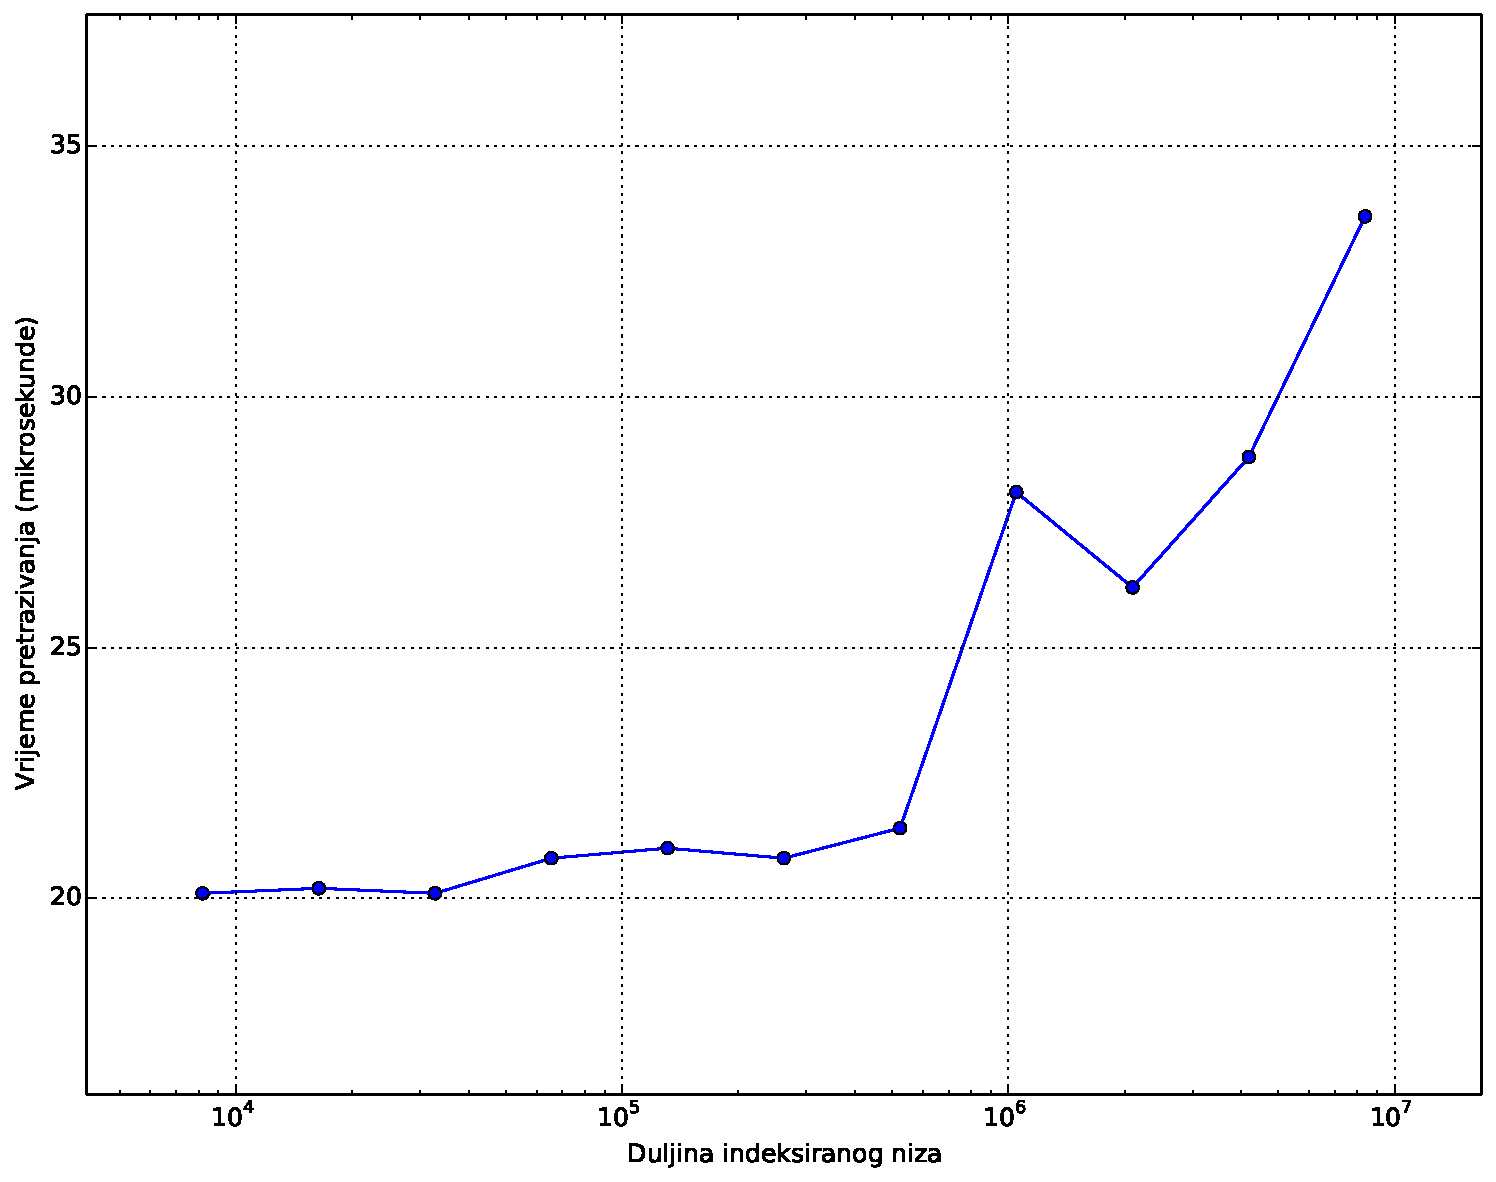
\includegraphics[width=\textwidth]{fig/test_res_seq_len.pdf}
\caption{Vrijeme pretraživanja u ovisnosti o duljini indeksiranog niza.}
\label{fig:test_res_seq_len_time}
\end{figure}

Rezultati su pomalo iznenađujući, s obzirom na teorijsko razmatranje konstantne složenosti
pretraživanja s obzirom na duljinu indeksiranog niza. U \cite{singer_2012} je observiran
isti fenomen, a objašnjen je kao posljedica hardverskog baratanja priručnom memorijom. Pri indeksiranju
nizova vrlo velike duljine, memorijski zahtjevi strukture indeksa postaju preveliki da bi
te strukture stale u priručnu memoriju. Prijenos podataka preko raznih razina priručne memorije
vremenski je zahtjevan i stoga snažno utječe na performase pretraživanja.

Slika \ref{fig:test_res_query_len_time} prikazuje trajanje pretraživanja
s obzirom na duljinu niza koji se traži (query). Testiranje je rađeno nad genomom
bakterije \textit{Escherichia coli}. Rezultati su srednje vrijednosti $10^5$ pretraga.

\begin{figure}[!htb]
\centering
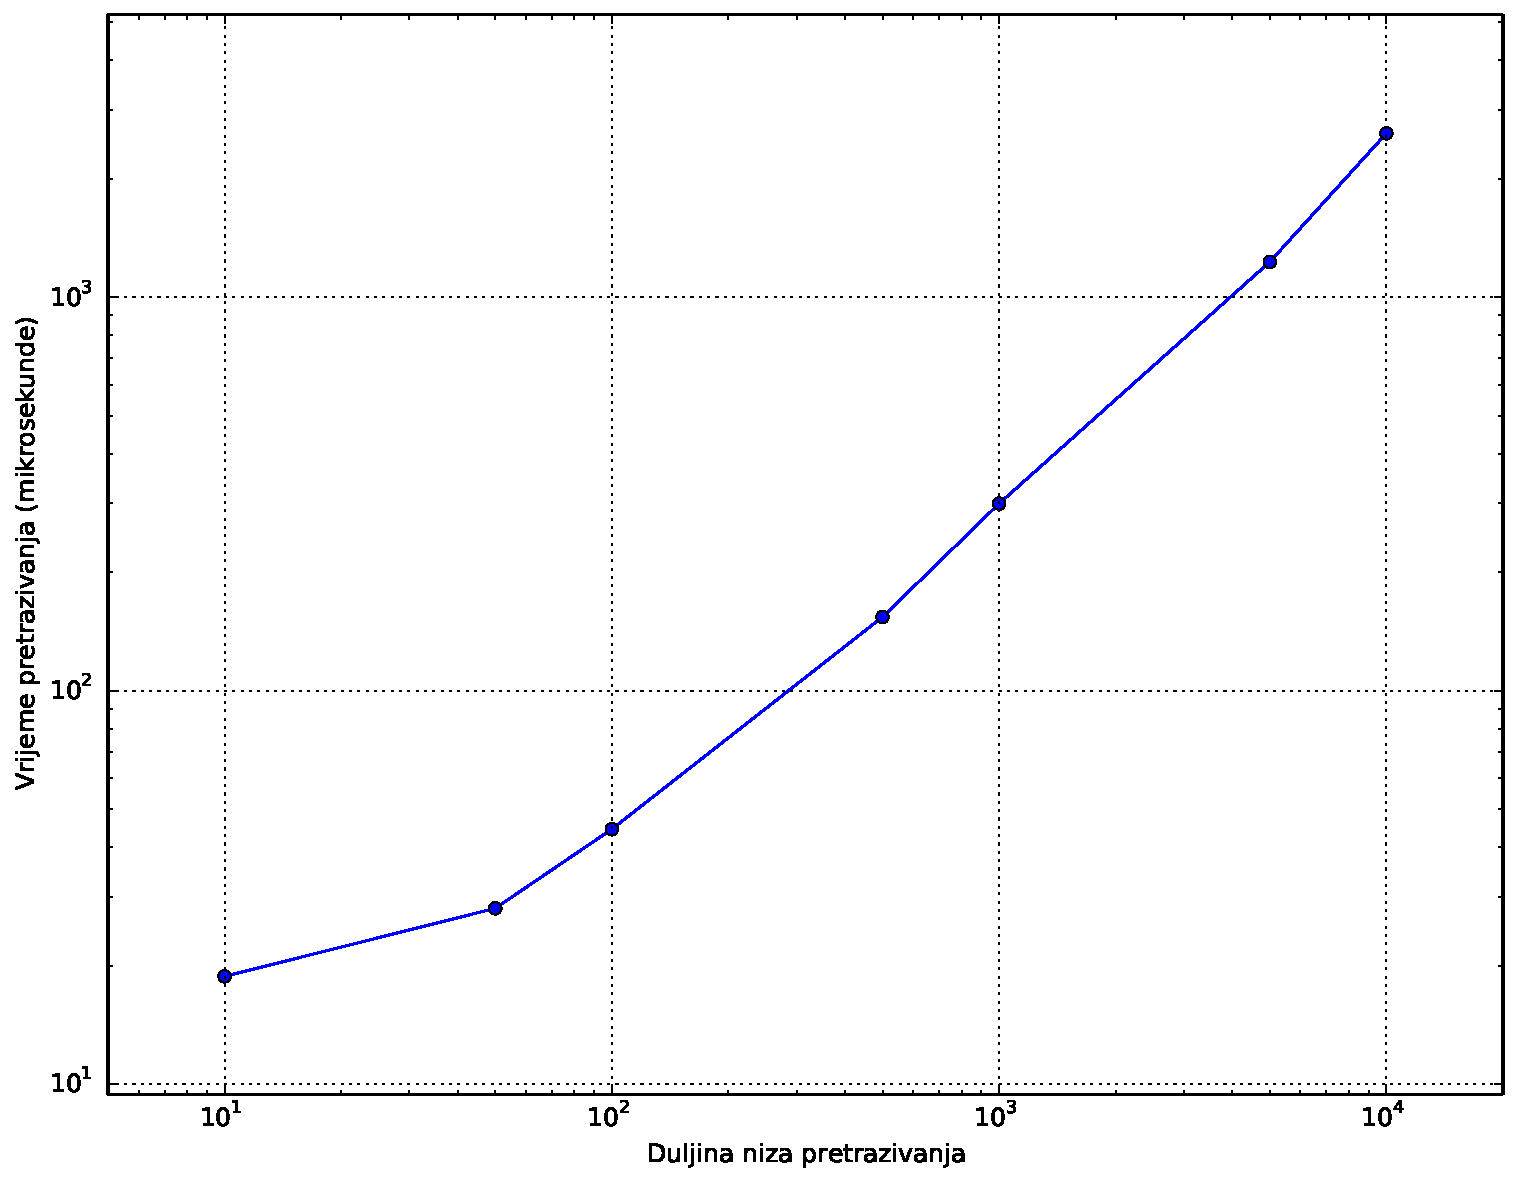
\includegraphics[width=\textwidth]{fig/test_res_query_len.pdf}
\caption{Vrijeme pretraživanja u ovisnosti o duljini indeksiranog niza.}
\label{fig:test_res_query_len_time}
\end{figure}

Rezultati su u skladu sa teorijskom analizom složenosti. Vidimo linearni porast
trajanja pretrage s obzirom na duljinu niza koji se pretražuje.

\subsubsection{Memorijska složenost}

Utrošak memorije na potporne strukture FM-indeksa prikazan je na slici \ref{fig:test_res_seq_len_mem}.
Testiranje memorije je rađeno sa istim podatcima kao i testiranje vremena trajanja pregrage.

\begin{figure}[!htb]
\centering
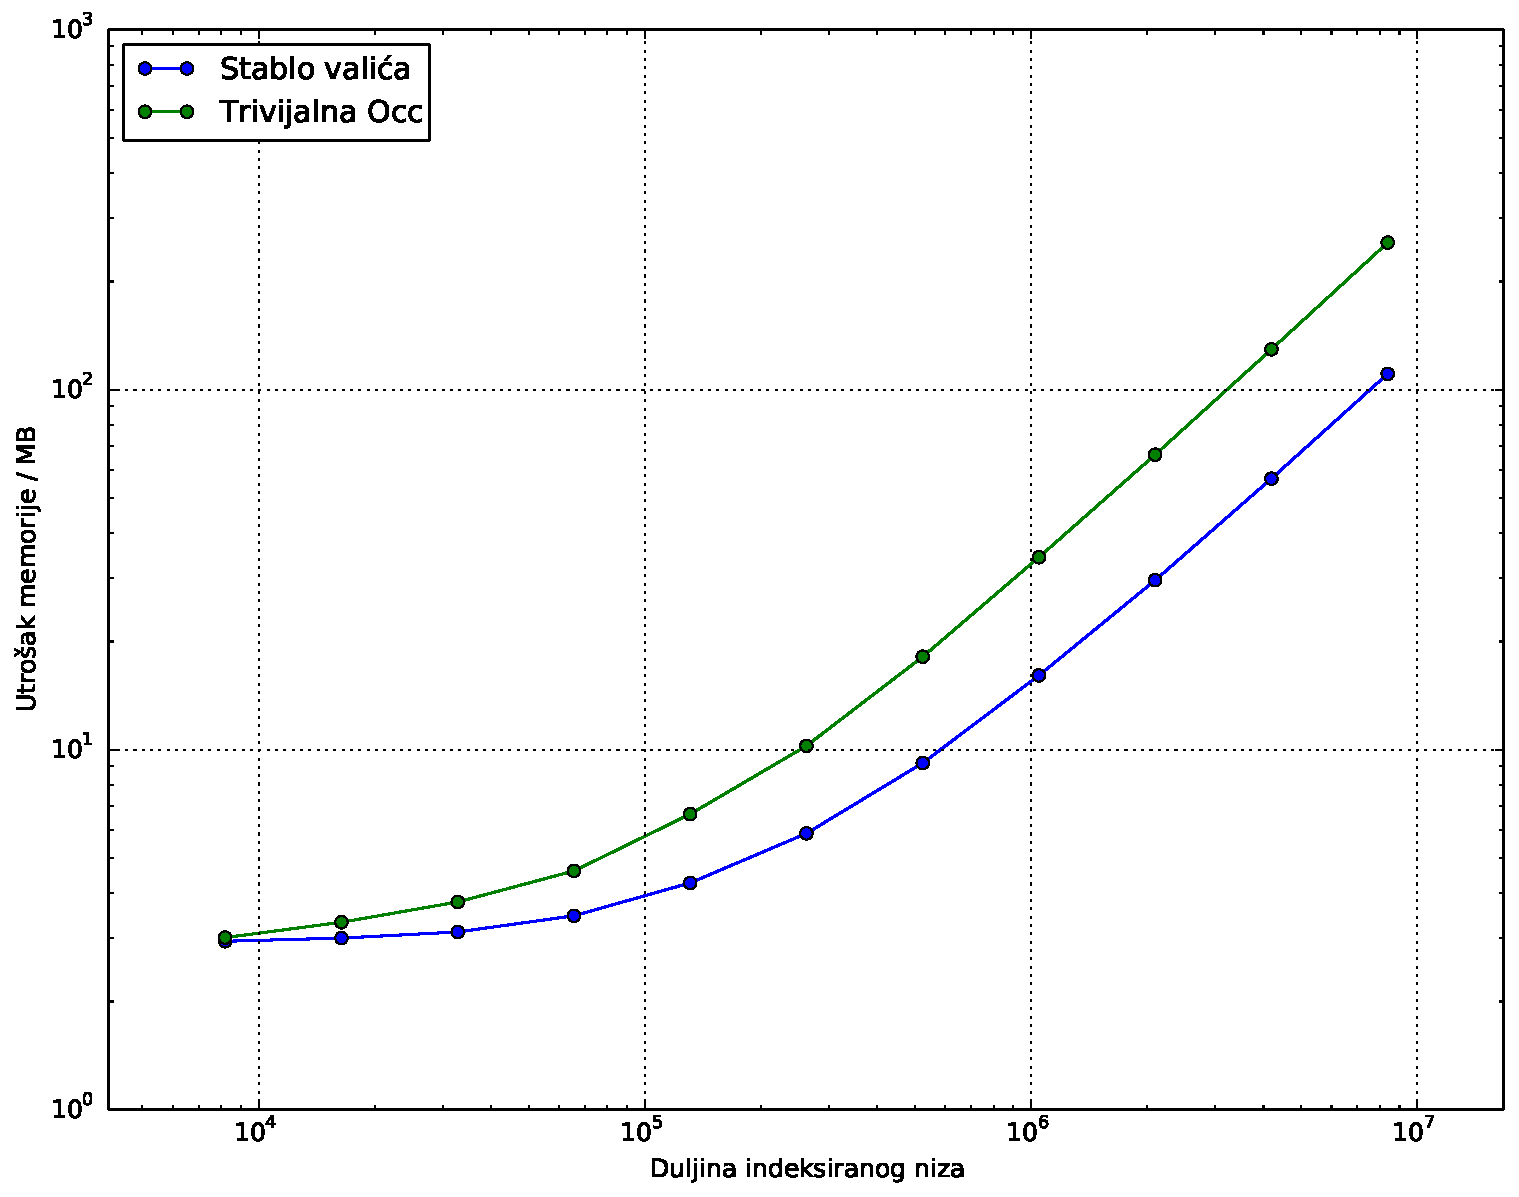
\includegraphics[width=\textwidth]{fig/test_res_seq_len_mem.pdf}
\caption{Utrošak memorije u ovisnosti o duljini indeksiranog niza.}
\label{fig:test_res_seq_len_mem}
\end{figure}

Iz grafa \ref{fig:test_res_seq_len_mem} vidljivo je kako je utrošak memorije s obzirom na
duljinu indeksiranog niza asimptotski linearan (primjetimo da su obje osi grafa logaritamske skale).
Rezultati su u skladu sa teorijskim razmatranjem memorijske potrošnje FM-indeks struktura podataka.

\chapter{Zaključak}
Zaključak.

\bibliography{literatura}
\bibliographystyle{unsrt}

\chapter{Sažetak}
Sažetak.

\end{document}
